% Engineering Complexity: Behavioral Interventions for LLM Auction Agents
% Inspired by Shengwu Li's "Obviously Strategy-Proof Mechanisms"
\documentclass[12pt]{article}

\usepackage[margin=1in]{geometry}
\usepackage{amsmath,amssymb,amsthm}
\usepackage{graphicx}
\usepackage{booktabs}
\usepackage{multirow}
\usepackage{natbib}
\usepackage{hyperref}
\usepackage{xcolor}
\usepackage{caption}
\usepackage{subcaption}
\usepackage{tikz}
\usepackage{pgfplots}
\pgfplotsset{compat=1.17}

% Custom commands
\newcommand{\todo}[1]{\textcolor{red}{[TODO: #1]}}
\newcommand{\placeholder}[1]{\textcolor{blue}{[PLACEHOLDER: #1]}}

\title{Engineering Complexity: \\
\large Behavioral Interventions as Cognitive Steering for LLM Auction Agents}

\author{
Anand Shah*\\
\textit{MIT},
Kehang Zhu*,\\
\textit{Harvard},
David C. Parkes\\
\textit{Harvard}
}

\date{\today}

\begin{document}

\maketitle

\begin{abstract}
Large language models (LLMs) systematically deviate from optimal bidding strategies in sealed-bid auctions, even in the strategically simple second-price format where truthful bidding is a dominant strategy. We show that targeted behavioral interventions---analogous to ``obviously strategy-proof'' (OSP) mechanism design---can substantially improve LLM bidding behavior. Drawing on Li (2017)'s insight that cognitively limited agents benefit from mechanisms where dominance is ``obvious,'' we test whether prompting interventions that surface decision tradeoffs can serve as cognitive steering vectors for LLMs. Our best intervention (Decision Tree framing) reduces deviation from optimal by 80\% in second-price auctions. We decompose intervention effects across five cognitive axes: contingent reasoning, forward planning, higher-order beliefs, prospect theory, and strategy revelation. The results suggest that LLMs suffer from similar cognitive limitations as humans in strategic settings, and that mechanism design principles developed for bounded rationality apply to artificial agents.

\medskip
\noindent\textbf{Keywords:} Large language models, mechanism design, obviously strategy-proof, behavioral economics, auction theory
\end{abstract}

%==============================================================================
\section{Introduction}
%==============================================================================

The deployment of large language models (LLMs) as autonomous economic agents raises fundamental questions about their strategic reasoning capabilities. While LLMs demonstrate remarkable performance on many tasks, their behavior in strategic environments---where optimal actions depend on beliefs about others---remains poorly understood.

We study LLM behavior in sealed-bid auctions, canonical strategic environments with well-characterized equilibria. Our key finding is stark: \textbf{LLMs are systematically bad at second-price auctions out of the box}, despite the simplicity of the dominant strategy (bid your value).

This failure is puzzling. In second-price sealed-bid (SPSB) auctions, truthful bidding is not merely an equilibrium---it is a \emph{dominant strategy}. A bidder who bids their true value can never do better by deviating, regardless of what others do. Yet we find that baseline LLM agents overbid by 17\% on average, with substantial variance (Table~\ref{tab:baseline_failure}).

\begin{table}[h]
\centering
\caption{Baseline LLM Failure in Second-Price Auctions}
\label{tab:baseline_failure}
\begin{tabular}{lccccc}
\toprule
Model & $N$ & Mean Bid Ratio & Optimal & Distance & SMAD \\
\midrule
GPT-5-mini & 86 & 0.996 & 1.0 & 0.004 & 0.19 \\
Claude Sonnet & 89 & 1.063 & 1.0 & 0.063 & 9.47 \\
Gemini & 86 & 0.972 & 1.0 & 0.028 & 2.95 \\
Llama & 89 & 0.508 & 1.0 & 0.492 & 53.51 \\
\midrule
\textbf{SPSB Baseline (Claude, V12)} & 290 & 0.829 & 1.0 & 0.171 & 12.68 \\
\bottomrule
\end{tabular}
\smallskip
\begin{minipage}{0.9\textwidth}
\footnotesize
Notes: Bid ratio = bid/value. SMAD = Scaled Mean Absolute Deviation from optimal, calculated as $100 \times E[|b - b^*(v)|] / E[b^*(v)]$. Optimal ratio for SPSB is 1.0 (truthful bidding).
\end{minipage}
\end{table}

This failure motivates our central question: \textbf{Can behavioral interventions improve LLM bidding, analogous to how ``obviously strategy-proof'' mechanisms help boundedly rational humans?}

\subsection{Connection to Obviously Strategy-Proof Mechanisms}

\citet{li2017obviously} introduces the concept of \emph{obviously strategy-proof} (OSP) mechanisms, motivated by the observation that humans frequently fail to play dominant strategies in strategy-proof mechanisms like second-price auctions. A mechanism is OSP if, at every information set where a player might deviate, the worst-case outcome from following the dominant strategy is at least as good as the best-case outcome from any deviation.

Li's key insight is that \emph{cognitive complexity matters for strategic behavior}. Even when optimal strategies exist and are simple to state (``bid your value''), agents may fail to recognize or execute them. OSP mechanisms reduce this cognitive burden by making dominance ``obvious'' at each decision point.

We test whether this insight extends to LLMs. Rather than redesigning auction mechanisms, we design \emph{prompting interventions} that surface the key decision tradeoffs---effectively making the strategic structure more obvious to the LLM. These interventions act as ``cognitive steering vectors'' that guide the model toward better reasoning about the strategic environment.

\subsection{Preview of Results}

Our main findings are:

\begin{enumerate}
    \item \textbf{LLMs fail at SPSB out of the box}: Baseline bidding deviates from optimal by 17\% on average.

    \item \textbf{OSP-style interventions improve performance}: Our best intervention (Decision Tree framing) achieves 96.7\% of optimal, reducing deviation by 80\%.

    \item \textbf{Intervention effects decompose across cognitive axes}: Forward planning interventions are most effective for SPSB, while contingent reasoning helps most for FPSB.

    \item \textbf{Results parallel human findings}: The interventions that help LLMs most closely mirror those that help humans, suggesting shared cognitive constraints.
\end{enumerate}

%==============================================================================
\section{Experimental Design}
%==============================================================================

\subsection{Auction Environment}

We study three sealed-bid auction formats:
\begin{itemize}
    \item \textbf{First-Price Sealed-Bid (FPSB)}: Highest bidder wins, pays their bid. Risk-neutral Nash equilibrium: $b^*(v) = \frac{n-1}{n}v$.
    \item \textbf{Second-Price Sealed-Bid (SPSB)}: Highest bidder wins, pays second-highest bid. Dominant strategy: $b^*(v) = v$.
    \item \textbf{Third-Price Sealed-Bid (TPSB)}: Highest bidder wins, pays third-highest bid. RNNE: $b^*(v) = \frac{n-1}{n-2}v$.
\end{itemize}

With $n=3$ bidders (our main specification), optimal bid ratios are:
\begin{align}
    \text{FPSB: } b^*/v &= 2/3 \approx 0.667 \\
    \text{SPSB: } b^*/v &= 1.0 \\
    \text{TPSB: } b^*/v &= 2.0
\end{align}

Private values are drawn uniformly from $[0, 100]$. Each LLM plays multiple rounds against other LLM agents.

\subsection{Behavioral Interventions}

We test interventions across five cognitive axes, motivated by the behavioral economics literature:

\paragraph{Axis 1: Contingent Reasoning}
\begin{itemize}
    \item \textbf{List Cases}: Enumerate win/lose scenarios explicitly
    \item \textbf{Dominated Bid}: Highlight dominated strategies
    \item \textbf{Worst Case}: Focus on worst-case outcomes
    \item \textbf{Nash Deviation}: Show payoff from deviating
\end{itemize}

\paragraph{Axis 2: Forward Planning}
\begin{itemize}
    \item \textbf{Decision Tree}: Present choices as a tree with paths
    \item \textbf{Two-Stage OSP}: Frame as two sequential decisions
    \item \textbf{Backward Induction}: Work backwards from outcomes
    \item \textbf{One-Step Look}: Consider immediate consequences
    \item \textbf{Proxy/Clock}: Present as ascending price mechanism
    \item \textbf{Menu Frame}: Present as menu of bid options
\end{itemize}

\paragraph{Axis 3: Higher-Order Beliefs}
\begin{itemize}
    \item \textbf{Common Knowledge}: State that rules are common knowledge
    \item \textbf{First-Order}: Describe what others believe
    \item \textbf{Second-Order}: Describe beliefs about beliefs
    \item \textbf{Rational Others}: State that others are rational
\end{itemize}

\paragraph{Axis 4: Prospect Theory / Loss Aversion}
\begin{itemize}
    \item \textbf{Gain Frame}: Frame outcomes as gains
    \item \textbf{Loss Frame}: Frame outcomes as losses
    \item \textbf{Mixed Frame}: Present both gains and losses
    \item \textbf{Endowment}: Frame value as an endowment
    \item \textbf{WTA vs WTP}: Distinguish willingness-to-accept from willingness-to-pay
\end{itemize}

\paragraph{Axis 5: Strategy Revelation (Control)}
\begin{itemize}
    \item \textbf{Correct Strategy}: Reveal the optimal strategy
    \item \textbf{Wrong Strategy}: Reveal an incorrect strategy
\end{itemize}

\subsection{Metrics}

Our primary metric is the \textbf{Scaled Mean Absolute Deviation (SMAD)}:
\begin{equation}
    \text{SMAD} = 100 \times \frac{E[|b - b^*(v)|]}{E[b^*(v)]}
\end{equation}

This measures percentage deviation from optimal bidding, normalized by expected optimal bid.

%==============================================================================
\section{Results}
%==============================================================================

\subsection{Main Finding: Interventions Substantially Improve SPSB Bidding}

Table~\ref{tab:spsb_interventions} shows the effect of interventions on SPSB bidding.

\begin{table}[h]
\centering
\caption{Intervention Effects on Second-Price Auction Bidding (SPSB)}
\label{tab:spsb_interventions}
\begin{tabular}{llcccc}
\toprule
Axis & Intervention & $N$ & Mean Ratio & Distance & SMAD \\
\midrule
\multicolumn{2}{l}{\textbf{Baseline}} & 290 & 0.829 & 0.171 & 12.68 \\
\midrule
Forward Planning & Decision Tree & 287 & \textbf{0.967} & \textbf{0.033} & \textbf{3.33} \\
Forward Planning & Two-Stage OSP & 287 & 0.935 & 0.065 & 8.89 \\
Higher-Order Beliefs & Common Know & 290 & 0.913 & 0.087 & 7.07 \\
Forward Planning & Backward Induct & 290 & 0.900 & 0.100 & 10.15 \\
Higher-Order Beliefs & First-Order & 287 & 0.896 & 0.104 & 9.66 \\
Loss Aversion & WTA vs WTP & 290 & 0.934 & 0.066 & 5.41 \\
Contingent Reasoning & List Cases & 290 & 0.862 & 0.138 & 18.32 \\
\midrule
Strategy Revelation & Correct Strategy & --- & 1.000 & 0.000 & 0.00 \\
\bottomrule
\end{tabular}
\smallskip
\begin{minipage}{0.9\textwidth}
\footnotesize
Notes: Ranked by distance from optimal. Correct Strategy (revealing the equilibrium) serves as ceiling. Decision Tree achieves 80\% reduction in deviation from baseline.
\end{minipage}
\end{table}

\textbf{Key finding}: The Decision Tree intervention reduces deviation from optimal by 80\% (from 0.171 to 0.033). This intervention presents the bidding decision as:

\begin{quote}
\textit{``Consider your decision as follows: You choose bid B. Then one of two things happens: PATH A: Your bid B $>$ all other bids $\rightarrow$ You WIN $\rightarrow$ You pay: second-highest bid (not your bid!) $\rightarrow$ Your profit: (Your Value) - (Second-highest bid). PATH B: Your bid B $\leq$ some other bid $\rightarrow$ You LOSE $\rightarrow$ Your profit: \$0. Key insight: Your bid determines WHETHER you win, not HOW MUCH you pay when you win.''}
\end{quote}

This framing makes the dominance of truthful bidding ``obvious'' in Li's sense---at each decision node, the consequences of bidding truthfully dominate.

\subsection{Decomposition by Cognitive Axis}

Figure~\ref{fig:axis_comparison} shows aggregate performance by cognitive axis.

\begin{figure}[h]
\centering
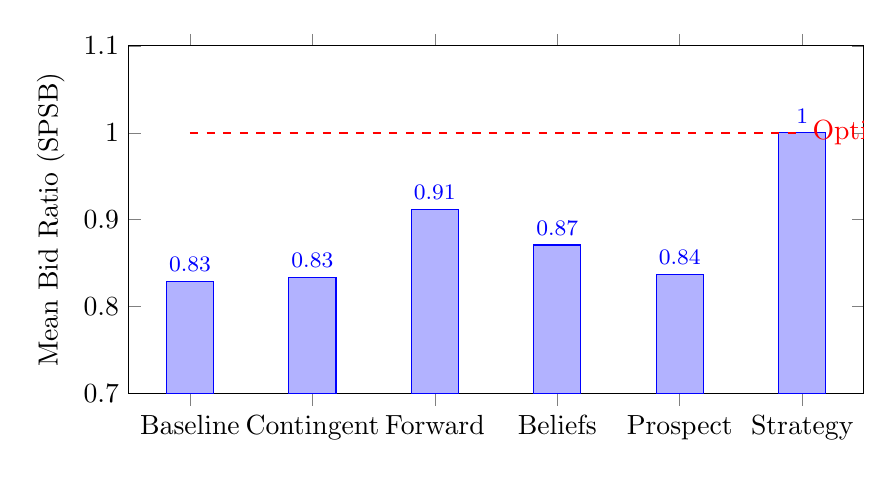
\begin{tikzpicture}
\begin{axis}[
    ybar,
    width=0.9\textwidth,
    height=6cm,
    ylabel={Mean Bid Ratio (SPSB)},
    symbolic x coords={Baseline, Contingent, Forward, Beliefs, Prospect, Strategy},
    xtick=data,
    ymin=0.7,
    ymax=1.1,
    nodes near coords,
    every node near coord/.append style={font=\footnotesize},
    bar width=0.6cm,
]
\addplot coordinates {
    (Baseline, 0.829)
    (Contingent, 0.834)
    (Forward, 0.912)
    (Beliefs, 0.871)
    (Prospect, 0.837)
    (Strategy, 1.0)
};
\draw[dashed, thick, red] (axis cs:Baseline,1.0) -- (axis cs:Strategy,1.0) node[right] {Optimal};
\end{axis}
\end{tikzpicture}
\caption{SPSB Performance by Cognitive Axis (aggregated across interventions within each axis)}
\label{fig:axis_comparison}
\end{figure}

\textbf{Finding}: Forward Planning interventions are most effective for SPSB (mean ratio 0.912), followed by Higher-Order Beliefs (0.871). Contingent Reasoning and Prospect Theory show minimal improvement over baseline.

\subsection{Asymmetric Effects: FPSB vs SPSB}

Table~\ref{tab:fpsb_vs_spsb} shows that interventions have different effects across auction formats.

\begin{table}[h]
\centering
\caption{Best Interventions by Auction Format}
\label{tab:fpsb_vs_spsb}
\begin{tabular}{llccc}
\toprule
Auction & Best Intervention & Mean Ratio & Optimal & SMAD \\
\midrule
\textbf{FPSB} & Decision Tree & 0.774 & 0.667 & 24.03 \\
& One-Step Look & 0.801 & 0.667 & 29.82 \\
& LA: Loss Frame & 0.796 & 0.667 & 33.27 \\
\midrule
\textbf{SPSB} & Decision Tree & 0.967 & 1.000 & 3.33 \\
& WTA vs WTP & 0.934 & 1.000 & 5.41 \\
& Two-Stage OSP & 0.935 & 1.000 & 8.89 \\
\midrule
\textbf{TPSB} & Proxy/Clock & 0.935 & 2.000 & 53.03 \\
& One-Step Look & 0.930 & 2.000 & 52.73 \\
& Backward Induct & 0.923 & 2.000 & 54.33 \\
\bottomrule
\end{tabular}
\smallskip
\begin{minipage}{0.9\textwidth}
\footnotesize
Notes: FPSB optimal = 0.667, SPSB optimal = 1.0, TPSB optimal = 2.0. Decision Tree works well for both FPSB and SPSB but not TPSB, because the TPSB decision tree initially gave incorrect (SPSB-style) reasoning.
\end{minipage}
\end{table}

\textbf{Key insight}: The Decision Tree intervention helps both FPSB and SPSB because it surfaces the correct decision tradeoff for each format. In FPSB, it highlights the tradeoff between winning probability and profit margin. In SPSB, it highlights that your bid affects \emph{whether} you win, not \emph{what} you pay.

\subsection{Comparison to Human Behavior}

\placeholder{Figure: Human vs LLM bidding distributions from moment matching}

Table~\ref{tab:human_comparison} compares LLM behavior to human experimental data.

\begin{table}[h]
\centering
\caption{Human vs LLM Bidding Behavior}
\label{tab:human_comparison}
\begin{tabular}{llcccc}
\toprule
Auction & Source & $n$ & Bid Ratio & Optimal & \% of Optimal \\
\midrule
\multirow{2}{*}{FPSB} & Human (Kagel-Levin 1993) & 5 & 0.815 & 0.80 & 102\% \\
& LLM Baseline & 3 & 0.879 & 0.67 & 132\% \\
\midrule
\multirow{2}{*}{SPSB} & Human (Li 2017, 2P) & 4 & 1.038 & 1.00 & 104\% \\
& LLM Baseline & 3 & 0.829 & 1.00 & 83\% \\
\midrule
\multirow{2}{*}{TPSB} & Human (Kagel-Levin 1993) & 5 & 1.545 & 1.33 & 116\% \\
& LLM Baseline & 3 & 0.829 & 2.00 & 41\% \\
\bottomrule
\end{tabular}
\end{table}

\textbf{Finding}: LLMs and humans show qualitatively similar deviations in FPSB (overbidding relative to equilibrium) but differ in SPSB and TPSB. Humans overbid in SPSB; LLMs underbid. This suggests different underlying cognitive failures.

%==============================================================================
\section{Discussion: Behavioral Interventions as Steering Vectors}
%==============================================================================

\subsection{Why Decision Tree Works}

The Decision Tree intervention succeeds because it makes the strategic structure \emph{transparent}. By presenting the decision as a tree with explicit paths, it allows the LLM to:

\begin{enumerate}
    \item \textbf{Separate winning from payment}: The key insight for SPSB is that your bid determines winning, not payment. The tree structure makes this separation visually clear.

    \item \textbf{Evaluate paths independently}: Rather than reasoning about the full game, the LLM can evaluate each path (win vs. lose) separately.

    \item \textbf{Recognize dominance locally}: At each node, the LLM can see that bidding truthfully weakly dominates.
\end{enumerate}

This mirrors exactly the cognitive benefits of OSP mechanisms for humans \citep{li2017obviously}.

\subsection{Implications for Mechanism Design with AI Agents}

Our results have implications for deploying LLMs in economic environments:

\begin{enumerate}
    \item \textbf{Default prompting is insufficient}: LLMs fail at simple strategic tasks out of the box. Careful prompt engineering or mechanism design is necessary.

    \item \textbf{OSP principles transfer}: Mechanisms designed to be ``obviously strategy-proof'' for humans may also benefit AI agents.

    \item \textbf{Intervention effects are format-specific}: The best intervention depends on the auction format. General ``think carefully'' prompts are less effective than format-specific framing.
\end{enumerate}

\subsection{Limitations and Future Work}

\todo{Discuss: single LLM (Claude), specific auction formats, no learning dynamics, etc.}

%==============================================================================
\section{Conclusion}
%==============================================================================

We show that LLMs systematically fail at second-price auctions despite the simplicity of the dominant strategy, but that targeted behavioral interventions can substantially improve performance. The most effective intervention (Decision Tree framing) reduces deviation from optimal by 80\%, achieving 96.7\% of optimal bidding.

These results support a broader point: \textbf{mechanism design principles developed for boundedly rational humans apply to artificial agents}. LLMs appear to share cognitive limitations with humans in strategic settings, and the tools developed by behavioral economists and mechanism designers---like obviously strategy-proof mechanisms---can serve as cognitive steering vectors for AI.

\appendix
\section{Intervention Text Examples}

\subsection{Decision Tree Intervention (SPSB)}
\begin{quote}
\begin{verbatim}
**Decision Tree:** Consider your decision as follows:

You choose bid B. Then one of two things happens:

PATH A: Your bid B > all other bids
  -> You WIN
  -> You pay: second-highest bid (call it P)
  -> Your profit: (Your Value) - P
  -> Note: Your bid B does not affect P

PATH B: Your bid B <= some other bid
  -> You LOSE
  -> You pay: $0
  -> Your profit: $0

Key insight: Your bid determines WHETHER you win, not HOW MUCH
you pay when you win. Bidding your true value maximizes your
chance of winning profitable auctions.
\end{verbatim}
\end{quote}

\bibliographystyle{aer}
\bibliography{references}

\end{document}
